\documentclass[10pt,twocolumn]{article}

\usepackage[a4paper,margin=18mm,columnsep=6mm]{geometry}
\usepackage[T1]{fontenc}
\usepackage[utf8]{inputenc}
\usepackage{lmodern}
\usepackage{microtype}
\usepackage{amsmath}
\usepackage{booktabs}
\usepackage{graphicx}
\usepackage{siunitx}
\usepackage{cite}
\usepackage{url}
\usepackage[font=small,labelfont=bf]{caption}
\usepackage{balance}

\DeclareSIUnit{\million}{million}
\DeclareSIUnit{\annum}{a}
\graphicspath{{../figures/png/}}
\sisetup{
  detect-all,
  group-separator={\,},
  group-minimum-digits=4,
  per-mode=symbol
}
\setlength{\emergencystretch}{2em}

\title{EnergyPlus-Trained Surrogate Models for Hourly Heating and Cooling Demand of the Vienna Building Stock}
\author{Philipp Thunshirn\\
\small Affiliation to be inserted\\
\small Email to be inserted}
\date{}

\begin{document}
\maketitle

\begin{abstract}
This study develops an EnergyPlus-trained surrogate for the building stock of
Vienna. The stock comprises \SI{134.6}{\million\metre\squared} of gross floor
area and is represented by eight residential and non-residential cohorts
covering four construction periods. EnergyPlus is not applied to the city as a
single large thermal zone. Instead, each cohort is simulated as a
\SI{1000}{\metre\squared} reference archetype, and the resulting hourly useful
heating and cooling intensities are scaled by the cohort floor areas obtained
from Citiwatts. Two histogram gradient-boosting surrogate models reproduce the
EnergyPlus outputs. Each combines an on/off classifier with a demand-magnitude
regressor. Validation on complete calendar weeks excluded from training gives
hourly $R^2$ values of 0.959 for heating and 0.975 for cooling. After
floor-area-weighted aggregation, annual city demand differs from EnergyPlus by
$+1.7\%$ for heating and $-0.8\%$ for cooling, while peak demand is
underestimated by $6.7\%$ and $10.1\%$, respectively. The complete EnergyPlus
demand path for eight annual cohort simulations takes \SI{67.1}{\second} on the
test system. Surrogate inference for the same 70,080 cohort-hours takes
\SI{1.73}{\second}, corresponding to a speedup of approximately 39. The model
provides fast EnergyPlus-consistent demand profiles; building flexibility and
energy-system optimization are not considered.
\end{abstract}

\noindent\textbf{Keywords:} EnergyPlus; building stock; surrogate model; space
heating; cooling; Vienna

\section{Introduction}

Hourly heating and cooling profiles are an important input to energy-system
models with high shares of renewable energy. Annual demand alone does not show
when heat pumps draw electricity, when heating coincides with a winter peak, or
when cooling increases the summer load. These questions require a building
model that responds to weather, solar and internal gains, occupancy schedules,
the thermal envelope, and the operation of the heating and cooling systems.
Simple degree-day relations or fixed normalized profiles can reproduce an
annual total, but they do not represent these interactions explicitly.

EnergyPlus provides a considerably richer description of building demand
\cite{crawley2001,doe2026}. It solves the transient heat balance and accounts
for heat transfer through opaque surfaces and windows, ventilation and
infiltration, solar radiation, internal gains, thermal storage, and HVAC
controls. Heating and cooling loads therefore follow from the same physical
balance instead of being imposed as independent profiles. EnergyPlus is also a
widely used and extensively documented building-performance simulation
program. This does not make every EnergyPlus result accurate by default:
geometry, material properties, schedules, and weather still have to represent
the case under study. Given suitable inputs, however, EnergyPlus offers a more
defensible basis for deriving hourly building loads than a profile assembled
from annual energy and outdoor temperature alone.

The detail that makes EnergyPlus useful also complicates its integration into
larger models. A city-scale application requires several representative
buildings, input files and schedules, repeated annual simulations, and the
extraction of results from EnergyPlus output files. Direct coupling becomes
particularly burdensome when building demand is evaluated repeatedly in
scenario analyses or optimization models. In such settings, the building
simulation can become a computational and technical bottleneck even when an
individual annual run is not prohibitively slow.

A surrogate model offers a practical division of work. EnergyPlus is retained
offline as the detailed teacher, while a statistical model learns the mapping
from weather, operating conditions, and building properties to useful heating
and cooling demand. Once trained, the surrogate can be called by an
energy-system model without constructing and executing a new EnergyPlus run
\cite{westermann2019,amasyali2018}. The gain in speed is only useful if annual
energy, hourly variation, seasonal transitions, and peak demand remain close to
the teacher simulation.

This paper demonstrates this approach for the Vienna building stock.
Citiwatts floor area and construction-period data are represented by eight
residential and non-residential cohorts. EnergyPlus simulations for the 2023
weather year provide hourly useful heating and cooling, which are emulated by a
gradient-boosting surrogate. The analysis addresses three questions: how
accurately the surrogate reproduces held-out hourly EnergyPlus results; whether
this accuracy is retained after aggregation to the Vienna stock, including
seasonal and peak periods; and how much computation time is saved. Building
flexibility, dispatch, and energy-system optimization are outside the scope.

\section{Materials and Methods}

\subsection{Case Study and Building-Stock Representation}

The case study covers the building stock within the Vienna boundary represented
in the Citiwatts inventory \cite{citiwatts2026}. The inventory reports a gross
floor area of \SI{134.6}{\million\metre\squared} and a heated volume of
\SI{403.7}{\million\metre\cubed}. Residential buildings account for
\SI{89.0}{\million\metre\squared} and non-residential buildings for
\SI{45.5}{\million\metre\squared}. Reported annual heat consumption is
\SI{17.54}{\tera\watt\hour\per\annum}. This value includes domestic hot water
and serves as a top-down energy-balance reference; it is distinct from the
useful space-heating output of the EnergyPlus simulations.

The stock was divided by sector and construction period. Residential and
non-residential buildings were each assigned to four periods: before 1975,
1975--1990, 1990--2000, and 2000--2014. The corresponding raw shares were 54\%,
24\%, 4\%, and 17\%, respectively, and were normalized before application
within each sector. The resulting eight cohorts sum to the complete Citiwatts
floor area. They represent an aggregation of the Vienna stock rather than a
sample of individual buildings.

Table~\ref{tab:cohorts} reports the floor-area weights and
period-dependent envelope parameters used in EnergyPlus. The U-value classes
are informed by Austrian TABULA/EPISCOPE apartment-building data
\cite{loga2016,aea2012}. In the absence of a corresponding Vienna
non-residential typology, the same construction-period classes were used for
both sectors. Residential solar transmittance values are proxies based on
comparable TABULA window classes; the non-residential models use a uniform
value of 0.60.

\begin{table*}[t]
\centering
\caption{Vienna stock weights and period-dependent envelope parameters.
The U-values are common to both sectors. Residential $g$-values are
cross-TABULA proxies; the uniform non-residential value is a model assumption.}
\label{tab:cohorts}
\scriptsize
\setlength{\tabcolsep}{4.0pt}
\resizebox{\textwidth}{!}{%
\begin{tabular}{lrrrrrrrr}
\toprule
&
\multicolumn{2}{c}{Represented floor area [\si{\million\metre\squared}]} &
\multicolumn{4}{c}{U-value [\si{\watt\per\metre\squared\per\kelvin}]} &
\multicolumn{2}{c}{Solar transmittance} \\
\cmidrule(lr){2-3}\cmidrule(lr){4-7}\cmidrule(lr){8-9}
Period &
$A_{\mathrm{res}}$ & $A_{\mathrm{nonres}}$ &
$U_{\mathrm{wall}}$ & $U_{\mathrm{win}}$ & $U_{\mathrm{roof}}$ & $U_{\mathrm{floor}}$ &
$g_{\mathrm{res}}$ & $g_{\mathrm{nonres}}$ \\
\midrule
$<1975$    & 48.6 & 24.8 & 1.40 & 2.30 & 1.70 & 1.20 & 0.85 & 0.60 \\
1975--1990 & 21.6 & 11.0 & 1.10 & 2.70 & 0.80 & 0.80 & 0.76 & 0.60 \\
1990--2000 &  3.6 &  1.8 & 0.60 & 2.50 & 0.50 & 0.50 & 0.60 & 0.60 \\
2000--2014 & 15.3 &  7.8 & 0.35 & 1.40 & 0.20 & 0.40 & 0.50 & 0.60 \\
\midrule
Total & 89.0 & 45.5 & \multicolumn{6}{c}{} \\
\bottomrule
\end{tabular}%
}
\end{table*}

Sector-specific geometry was retained outside the period classification.
For residential buildings, wall, window, roof, and exposed-floor areas were
0.82, 0.18, 0.37, and 0.36 m² per m² conditioned floor area, respectively.
The corresponding non-residential ratios were 0.30, 0.12, 0.30, and 0.30.
Residential areal heat capacities decreased from 80 to
\SI{65}{\watt\hour\per\metre\squared\per\kelvin} across the four periods;
non-residential values decreased from 70 to
\SI{55}{\watt\hour\per\metre\squared\per\kelvin}. The residential geometry is
TABULA-informed, whereas the non-residential geometry and all heat-capacity
values are explicit model assumptions.

Residential domestic-hot-water demand is estimated in the wider Vienna data
set at \SI{15.5}{\kilo\watt\hour\per\metre\squared\per\annum} and separated
from the inventory heat total. Domestic hot water is not simulated or
predicted in this study. Similarly, the annual Citiwatts heat consumption is
not a regression target. Citiwatts defines the stock extent and provides the
floor-area weights used for city aggregation. A subsequent energy-system
application may normalize the EnergyPlus-derived profile and apply an external
annual energy total, but this operation is not part of the validation below.

\subsection{EnergyPlus Reference Simulations}

One EnergyPlus 26.1 model was prepared for each cohort
\cite{doe2026}. The models represent equivalent stock archetypes rather than
particular buildings. A conditioned reference floor area of
\SI{1000}{\metre\squared} was used in all simulations. This common reference
area keeps the geometry at a plausible archetype scale and permits the output
to be expressed as demand intensity. It does not restrict the represented
stock to \SI{1000}{\metre\squared}. Envelope areas, internal gains, and air
volumes were scaled consistently with the reference area, so the resulting
specific demand can be applied to the corresponding cohort floor area.

The Citiwatts volume-to-area ratio gives a reference room height of
approximately \SI{3}{\metre} and a conditioned volume of approximately
\SI{3000}{\metre\cubed}. Each archetype was simulated for the 8760 hours of
2023. Outdoor temperature and solar radiation were obtained from Open-Meteo
and converted to a pseudo-EPW weather file \cite{zippenfenig2023}. A
Climate.OneBuilding file for Wien-Innere-Stadt supplied EPW header and format
information but not the hourly observations \cite{climateonebuilding}.
Heating and cooling setpoints were \SI{22}{\degreeCelsius} and
\SI{27}{\degreeCelsius}. The simulations included transmission through the
envelope, solar and internal gains, ventilation, infiltration, and ideal-load
heating and cooling. EnergyPlus returned hourly useful space-heating and
useful-cooling demand. The separate winter experiment shown in
Fig.~\ref{fig:teacher} illustrates heat-balance differences between
residential construction periods and was not added to the training data.

The outputs were converted to specific hourly demand
$q_{c,t}^{\mathrm{EP}}$ in \si{\kilo\watt\hour\per\metre\squared\per\hour}.
City-level demand was obtained by multiplying this intensity by the represented
floor area $A_c$ and summing across cohorts:
\begin{equation}
Q_{c,t}=q_{c,t}^{\mathrm{EP}}A_c,\qquad
Q_t^{\mathrm{Vienna}}=\sum_{c=1}^{8}Q_{c,t}.
\label{eq:aggregation}
\end{equation}
Equation~\eqref{eq:aggregation} represents the complete inventory area through
eight specific demand profiles. It is not a calibration of the EnergyPlus
annual sum to the \SI{17.54}{\tera\watt\hour} Citiwatts heat balance, which
includes end uses outside the EnergyPlus targets. The unnormalized EnergyPlus
series is retained so that teacher and surrogate are compared on the same
basis.

\subsection{Dataset Generation and Preprocessing}

Combining eight cohort simulations with 8760 time steps produced 70,080
observations. One observation describes one cohort during one hour. Two target
variables were derived: useful space-heating demand and useful cooling demand,
both in \si{\kilo\watt\hour\per\metre\squared\per\hour}. Separate models were
trained for the two targets.

The explanatory variables cover four parts of the EnergyPlus input:
\begin{itemize}
  \item \textit{weather}: outdoor-air temperature, global horizontal
  irradiation, direct normal irradiation, and diffuse horizontal irradiation;
  \item \textit{operation}: heating and cooling setpoints, internal gains,
  infiltration, and ventilation air-change rates;
  \item \textit{time}: sine and cosine transformations of hour of day and day
  of year; and
  \item \textit{building}: sector, cohort indicators, envelope U-values,
  envelope-area ratios, and areal heat capacity.
\end{itemize}
The periodic time transformations avoid artificial discontinuities between
hour 23 and hour 0 and between the end and beginning of the year.

A specific heat-loss coefficient was calculated from the products of U-values
and their corresponding envelope-area ratios. Heating and cooling temperature
differences were calculated between outdoor temperature and the respective
setpoint. Their products with the heat-loss coefficient were included as
additional variables. These engineered terms expose the principal thermal
driving forces to the tree ensemble without using an EnergyPlus result as an
input.

All cohort-hour combinations were retained; no random subsampling was applied.
Data preparation required eight complete annual profiles, checked for
duplicate cohort--timestamp pairs, and rejected missing values. Targets were
normalized by represented cohort area before fitting. Floor-area values were
used again only after prediction to obtain the city-level series.

\subsection{Surrogate Model}

Heating and cooling were modelled independently using the histogram-based
gradient-boosting implementation in scikit-learn
\cite{friedman2001,pedregosa2011,ke2017}. Gradient boosting constructs an
additive ensemble of decision trees in which each iteration reduces the
residual error of the current ensemble. This model class accommodates the
combination of continuous weather and envelope parameters, cyclic time
variables, and categorical cohort information used here.

Both targets contain long periods without demand. A single regression model
gave excessive influence to these hours and produced residual summer heating.
A two-part hurdle formulation was therefore used for each service. A
\texttt{HistGradientBoostingClassifier} first estimates the probability
$\widehat p_t$ that demand is present. A
\texttt{HistGradientBoostingRegressor} estimates the demand magnitude
$\widehat q_t^{\mathrm{reg}}$. During inference, the non-negative regression
output is retained if the probability exceeds a service-specific threshold
$\tau$:
\begin{equation}
\widehat q_t =
\begin{cases}
\max(0,\widehat q_t^{\mathrm{reg}}), & \widehat p_t \geq \tau,\\
0, & \widehat p_t < \tau.
\end{cases}
\label{eq:hurdle}
\end{equation}

Monotonic constraints were applied where the expected physical direction is
unambiguous. Predicted heating cannot increase with outdoor temperature and
increases with the heating temperature difference. Cooling follows the
opposite temperature response. Other variables remain unconstrained.

The regression component used a learning rate of 0.05, up to 700 boosting
iterations, at most 159 leaf nodes per iteration, and an L2 regularization
coefficient of 0.01. The classifier used up to 300 boosting iterations, 63 leaf
nodes, and an L2 coefficient of 0.05. These settings define the active v2
surrogate.

\subsection{Model Training and Validation}

All 70,080 observations entered the cross-validation procedure. Sample weights
prevented moderate- and zero-demand hours from dominating the regression loss.
Positive observations up to the median positive demand received weight 2,
whereas observations in the highest 15\% of positive demand received weight 9.
Remaining observations, including zero-demand hours, received weight 1. For
the classification component, positive and zero classes were balanced within
each training fold.

The hurdle threshold was selected independently in each training fold from
0.10 to 0.90 in increments of 0.05. The selection criterion retained energy
during true on-hours while penalizing demand during physically implausible
off-hours. These were hours with outdoor temperature at or above the heating
setpoint for heating, and at or below the heating setpoint for cooling.
Threshold selection used training-fold predictions only. The selected
threshold was 0.10 in all heating folds and ranged from 0.65 to 0.70 in the
cooling folds.

Temporal generalization was assessed by four-fold grouped cross-validation,
using the ISO calendar week as the grouping variable. All hours of a given
week, across all eight cohorts, were assigned to the same fold. Adjacent hours
were therefore not randomly divided between training and validation data, and
each reported prediction refers to a week excluded from the corresponding
fit. All cohorts were represented in each fold. The procedure evaluates unseen
periods within the 2023 weather year; it does not test a previously unseen
building class or an independent climate year.

Held-out cohort-hour predictions were evaluated with the coefficient of
determination ($R^2$), mean absolute error (MAE), and root mean squared error.
Predictions were subsequently scaled according to
Eq.~\eqref{eq:aggregation} to obtain a fully out-of-fold Vienna time series.
Annual relative error, peak-hour relative error, and Pearson correlation were
calculated for that series. The deployable models were finally refitted to the
complete annual data set; these full-data fits were not used to report
accuracy.

\subsection{Runtime Assessment}

Computational performance was measured for all eight annual cohort profiles on
one computer. The EnergyPlus path included schedule and IDF generation,
execution of the simulation engine, and extraction of hourly results from the
SQL output. Engine time was measured three times per cohort and aggregated
from the cohort medians. Inference for both surrogate targets was repeated five
times and the median duration was reported. Plot generation was disabled. The
one-time training duration was recorded separately and excluded from the
inference speedup.

\section{Results}

\subsection{EnergyPlus Cohort Response}

The EnergyPlus heat balances differ markedly between residential construction
periods (Fig.~\ref{fig:teacher}). During the selected winter day, approximate
transmission losses decline from about \SI{82}{\watt\per\metre\squared} for
the pre-1975 cohort to about \SI{26}{\watt\per\metre\squared} for the
2000--2014 cohort. Ventilation losses are similar because the same
air-change assumption is used across cohorts. Infiltration is omitted from the
figure because its common rate does not distinguish construction periods.

\begin{figure*}[t]
\centering
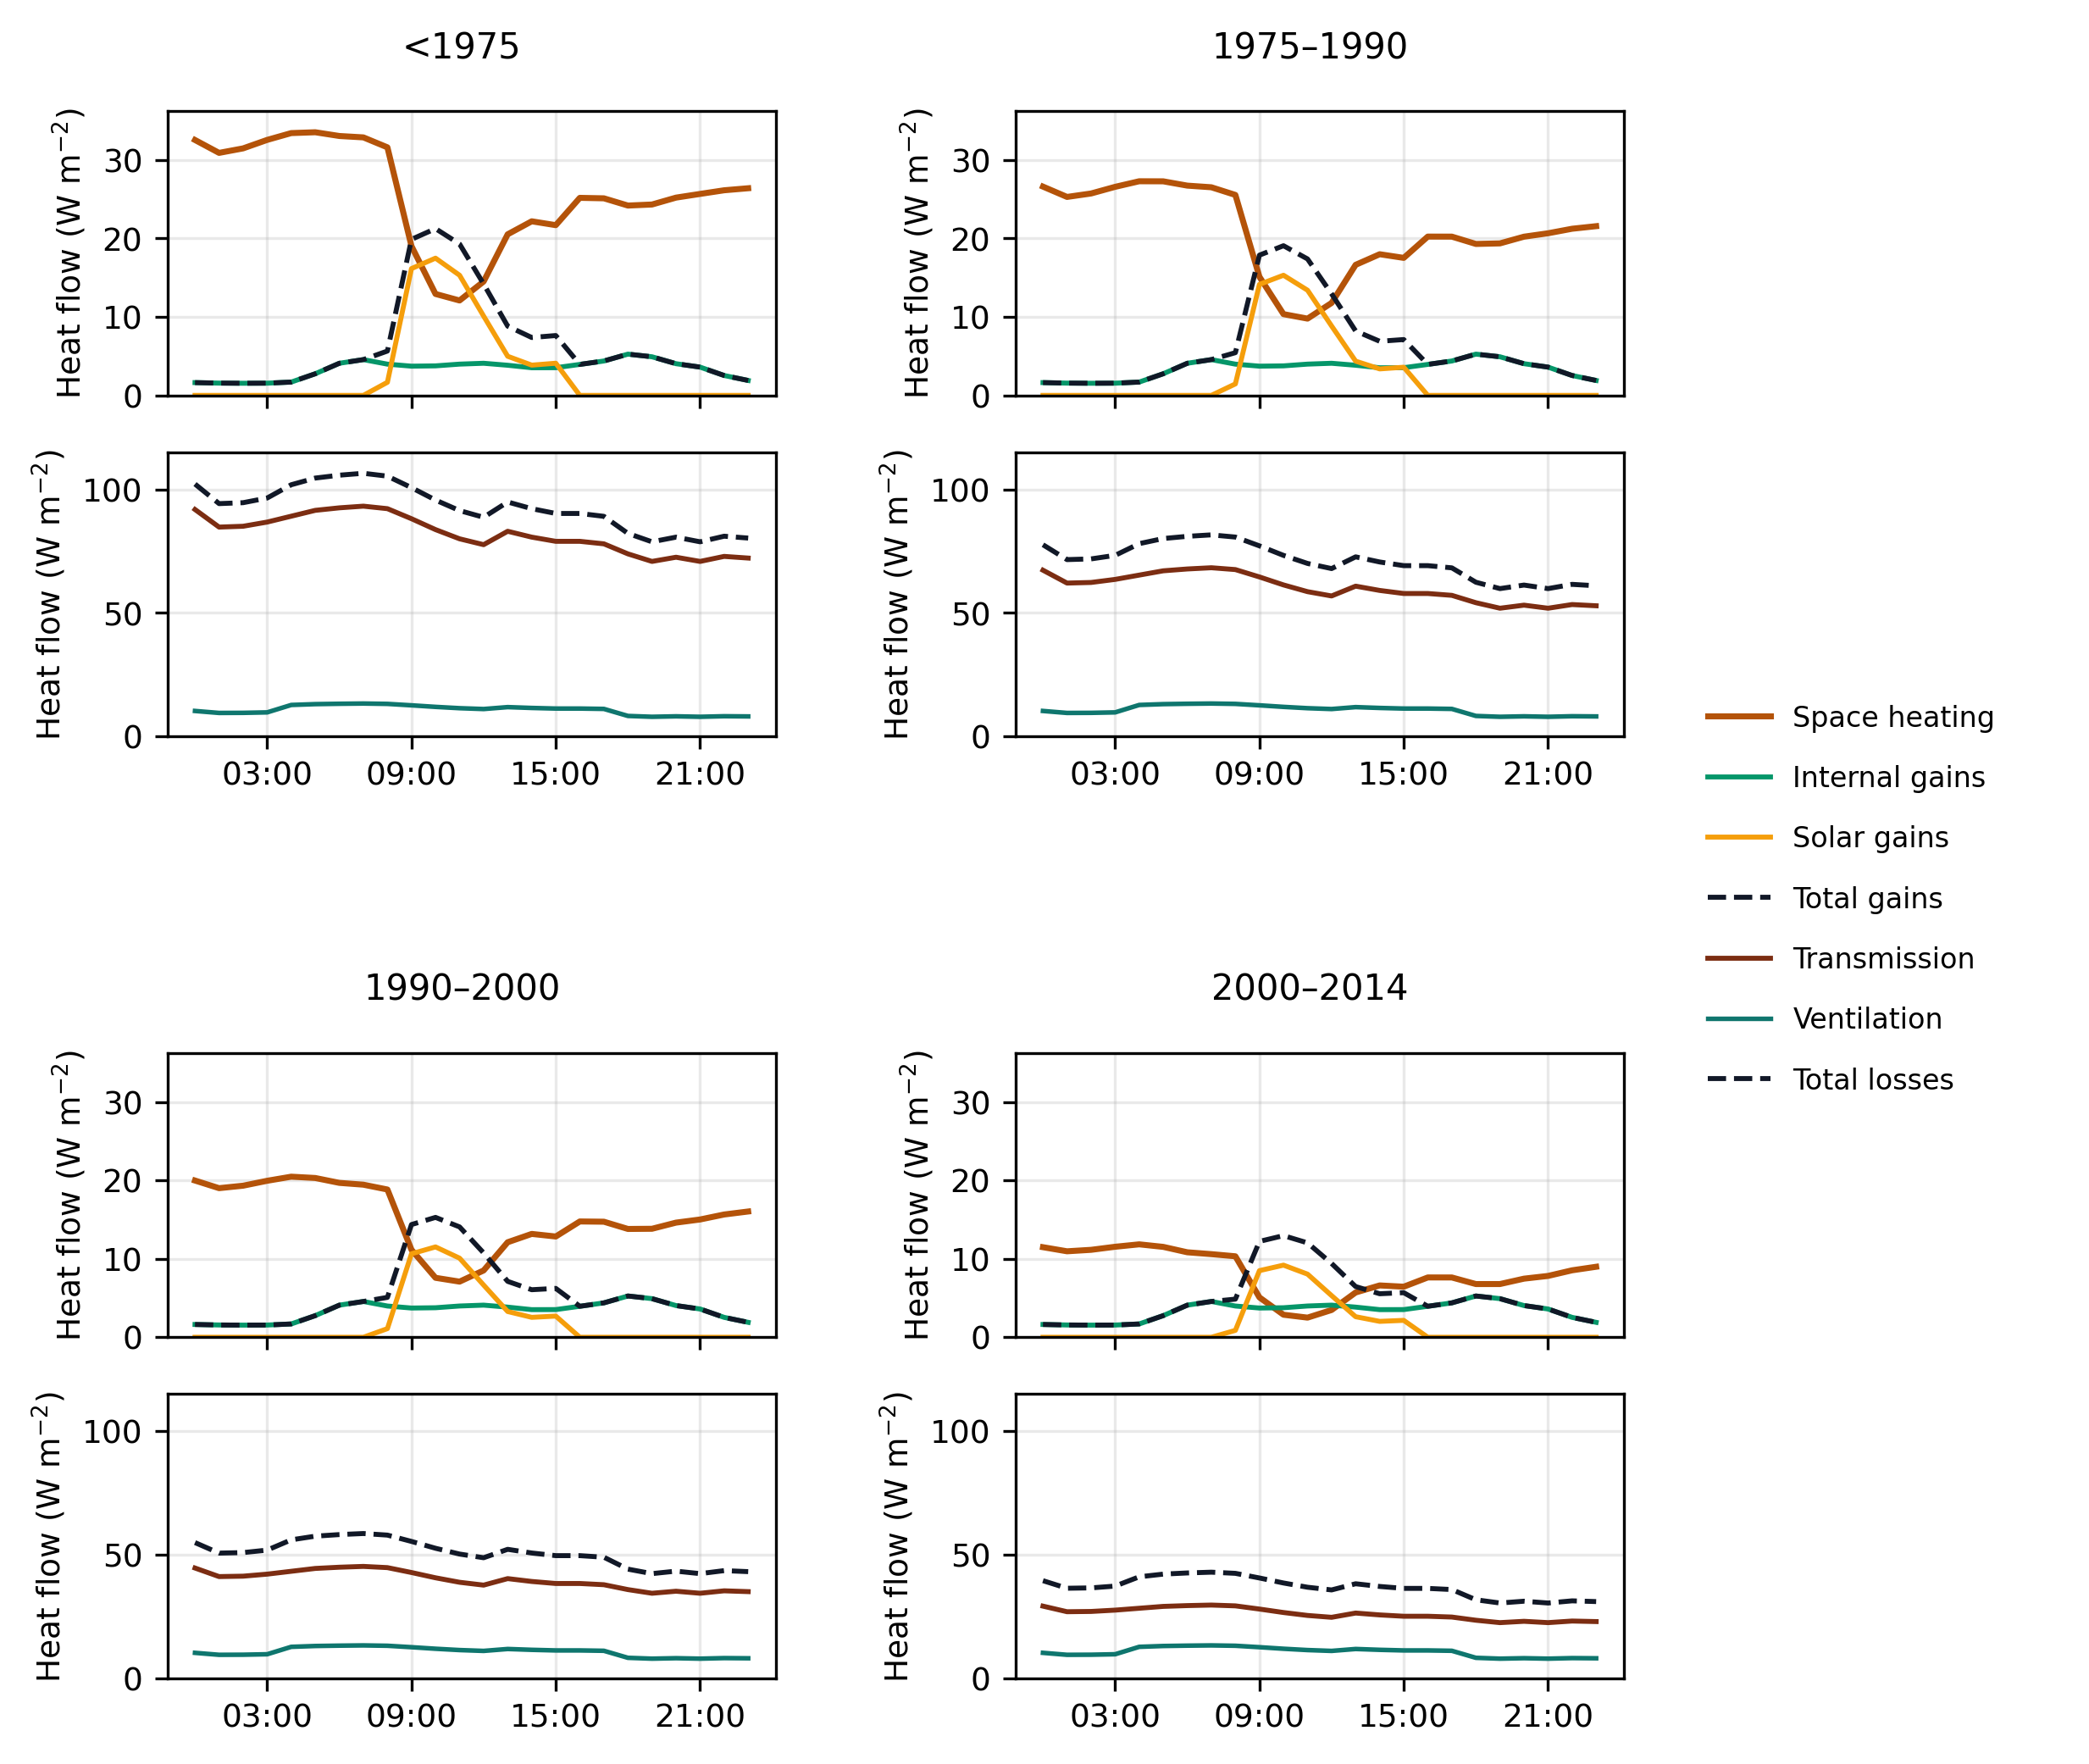
\includegraphics[width=\textwidth]{fig_01_teacher_flow_day.png}
\caption{EnergyPlus teacher heat-balance flows for four residential
construction periods during a winter day. Upper panels show space heating,
internal gains, solar gains, and total gains. Lower panels show approximate
transmission and ventilation losses. Common axis limits permit direct
comparison between construction periods.}
\label{fig:teacher}
\end{figure*}

\subsection{Surrogate Accuracy}

Table~\ref{tab:accuracy} summarizes the out-of-fold accuracy. At cohort-hour
level, the surrogate reaches an $R^2$ of 0.959 for heating and 0.975 for
cooling. After floor-area-weighted aggregation, annual city demand differs
from EnergyPlus by $+1.7\%$ for heating and $-0.8\%$ for cooling. The temporal
correlations of the city series are 0.982 and 0.989. The largest discrepancy
occurs at the annual maximum: peak heating is underestimated by 6.7\% and peak
cooling by 10.1\%.

\begin{table}[t]
\centering
\caption{Four-fold calendar-week cross-validation of the active surrogate.}
\label{tab:accuracy}
\small
\setlength{\tabcolsep}{4pt}
\begin{tabular}{lrr}
\toprule
Metric & Heating & Cooling \\
\midrule
Hourly $R^2$ & 0.959 & 0.975 \\
MAE [\si{\kilo\watt\hour\per\metre\squared\per\hour}]
  & $5.8{\times}10^{-4}$ & $5.4{\times}10^{-4}$ \\
City annual error [\%] & $+1.7$ & $-0.8$ \\
City peak-hour error [\%] & $-6.7$ & $-10.1$ \\
City Pearson $r$ & 0.982 & 0.989 \\
\bottomrule
\end{tabular}
\end{table}

Annual heating errors for the large residential cohorts remain within a few
percent. The largest cohort-relative error occurs for non-residential
buildings from 2000--2014 ($+23\%$). Their EnergyPlus heating intensity is only
\SI{3.8}{\kilo\watt\hour\per\metre\squared\per\annum}; consequently, a small
absolute deviation produces a large percentage error and has little influence
on the aggregate Vienna result. Annual cooling errors remain within
approximately $\pm2\%$ for all cohorts.

The selected seasonal weeks in Fig.~\ref{fig:weeks} show how the aggregate
error is distributed in time. During the peak-heating week, the surrogate
follows the daily variation but underestimates the highest loads; total heating
energy over the week is 1.6\% below EnergyPlus. In the early-April heating
week, energy is 3.5\% higher and the peak magnitude is closely reproduced.
Cooling profiles in late August and September show close agreement in most
hours. The absolute August cooling peak remains underestimated, consistent
with the annual peak metric.

\begin{figure*}[t]
\centering
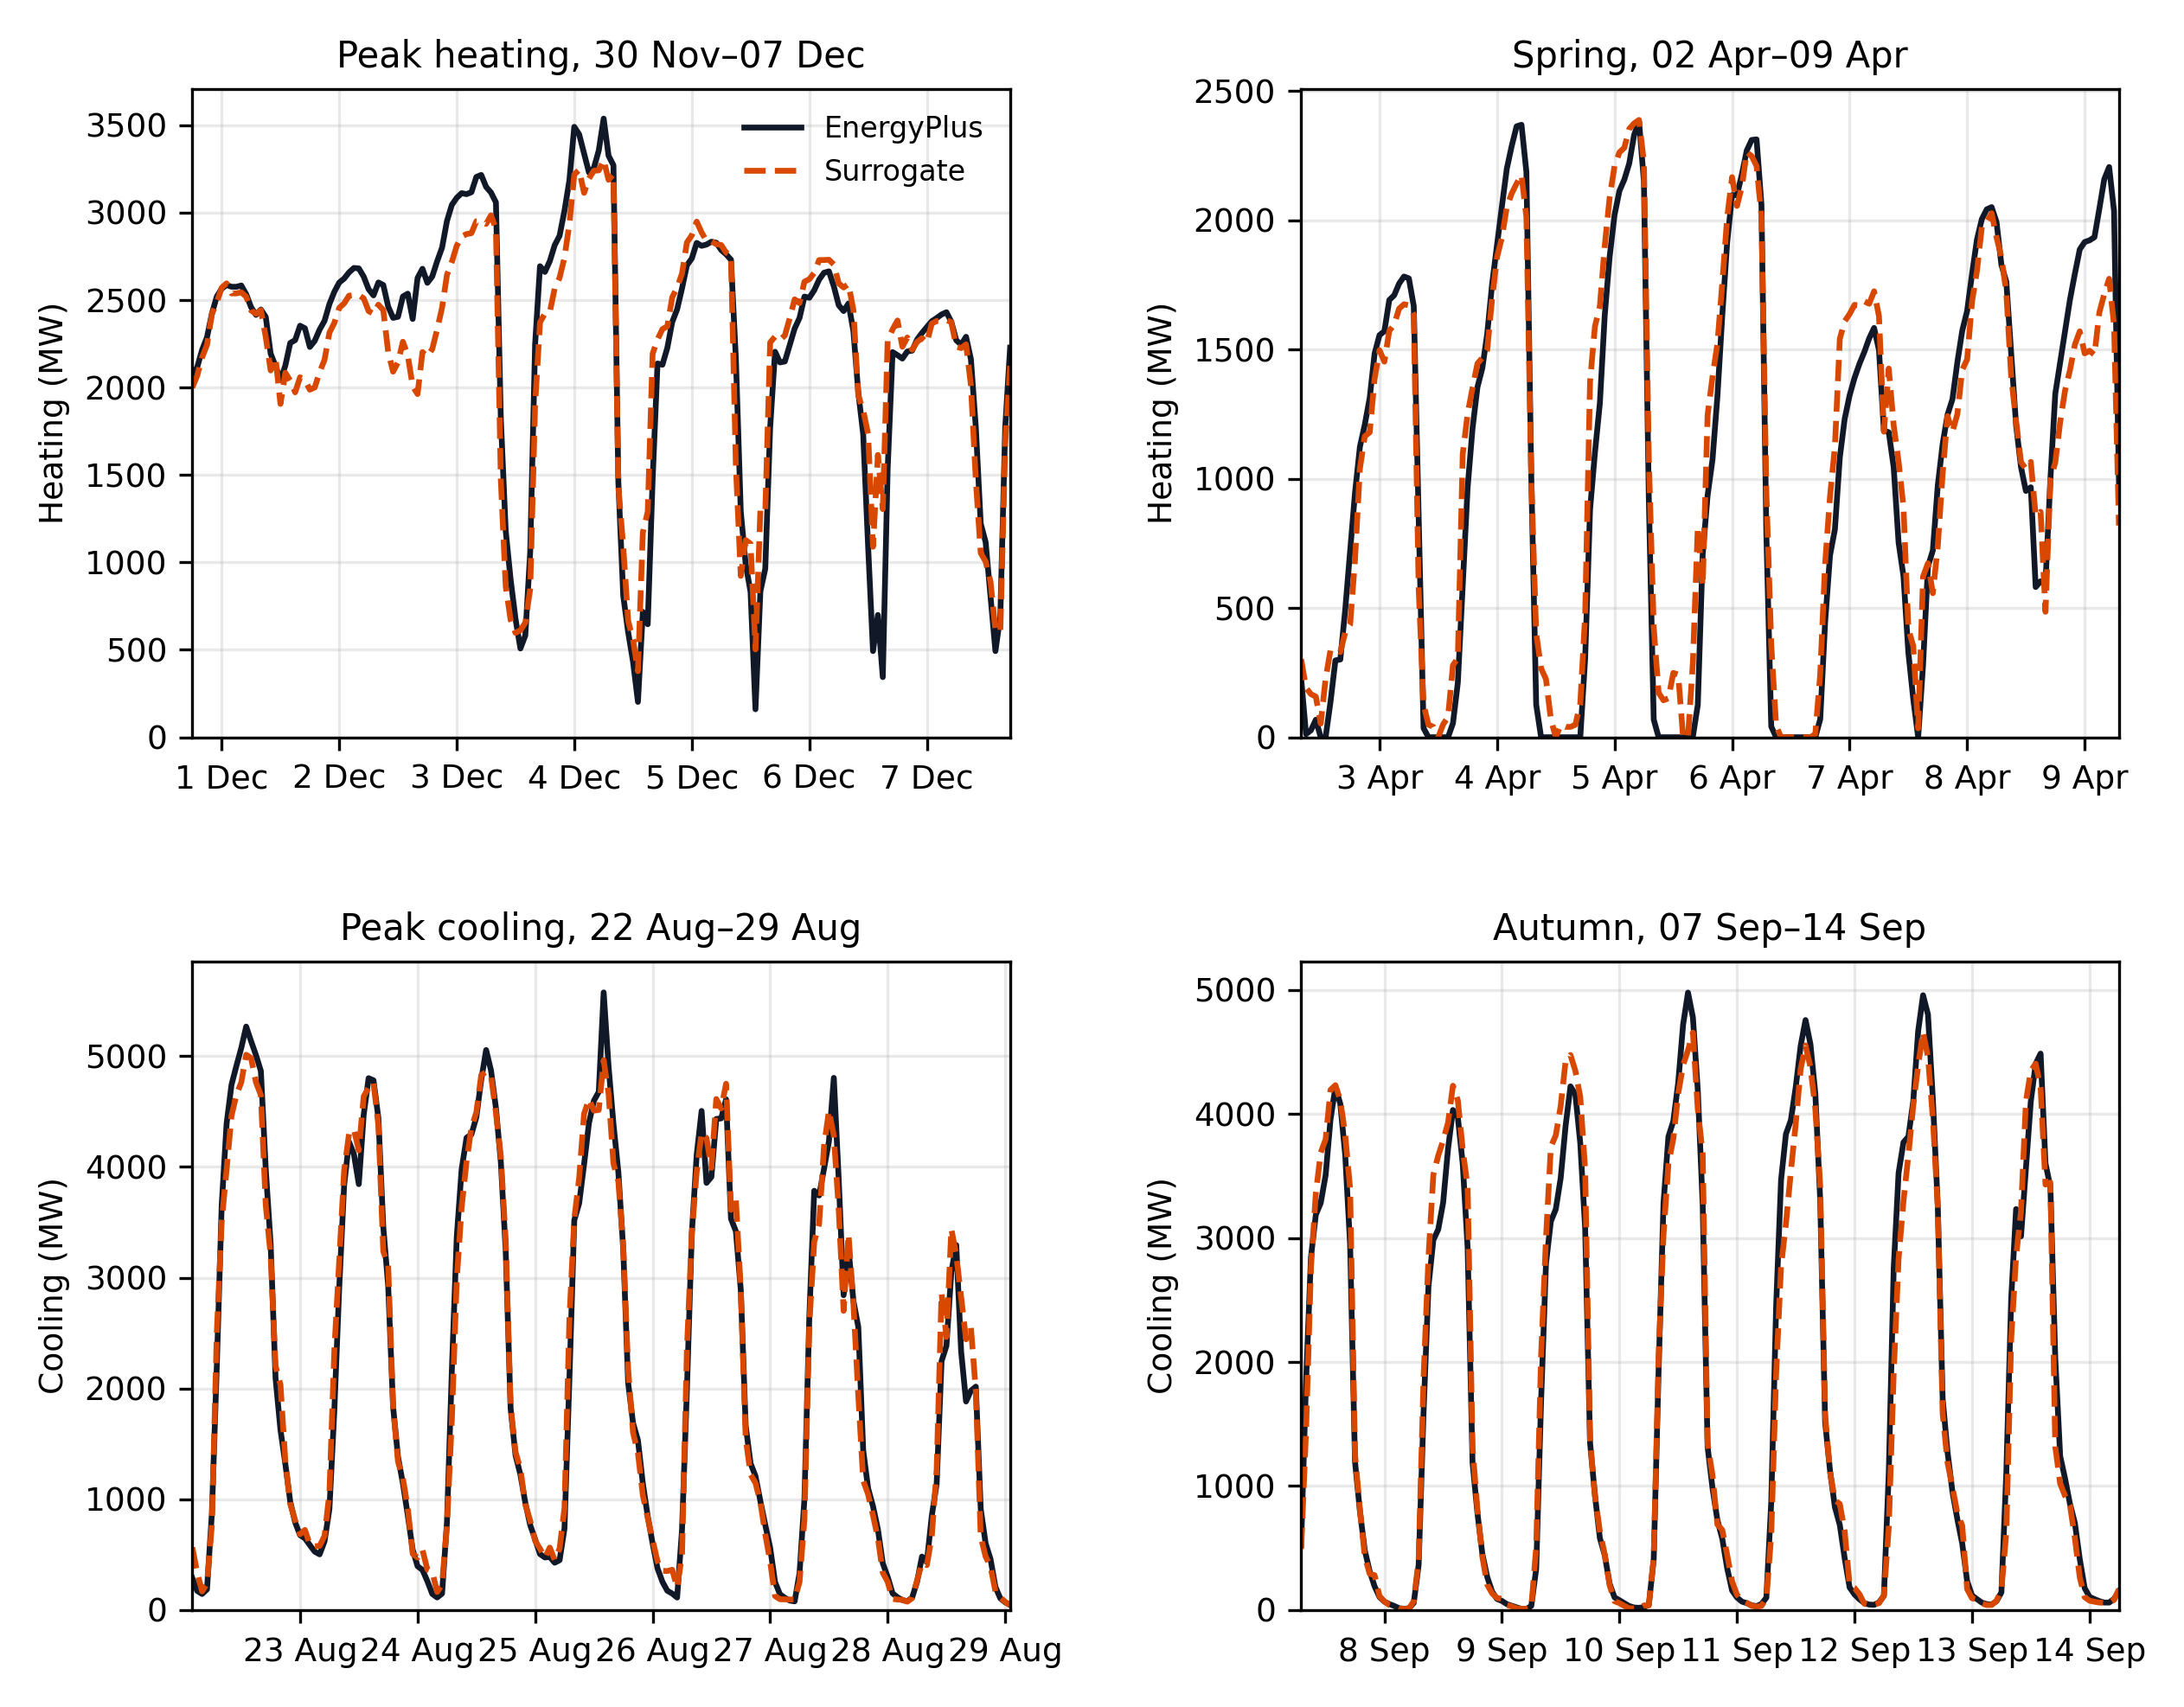
\includegraphics[width=0.96\textwidth]{fig_02_city_holdout_seasonal_weeks.png}
\caption{Floor-area-weighted Vienna useful demand from EnergyPlus and held-out
surrogate predictions. The panels show the peak-heating week, an April heating
week, the peak-cooling week, and a September cooling week. Each interval
contains 168 consecutive hours.}
\label{fig:weeks}
\end{figure*}

Figure~\ref{fig:temperature} relates city demand to outdoor temperature. The
1-K bin means produced by the surrogate follow those of EnergyPlus for both
services. Heating decreases as outdoor temperature rises, whereas cooling
increases at high temperatures. The transition between the two regimes is
retained without a substantial band in which both services are simultaneously
overpredicted.

\begin{figure*}[t]
\centering
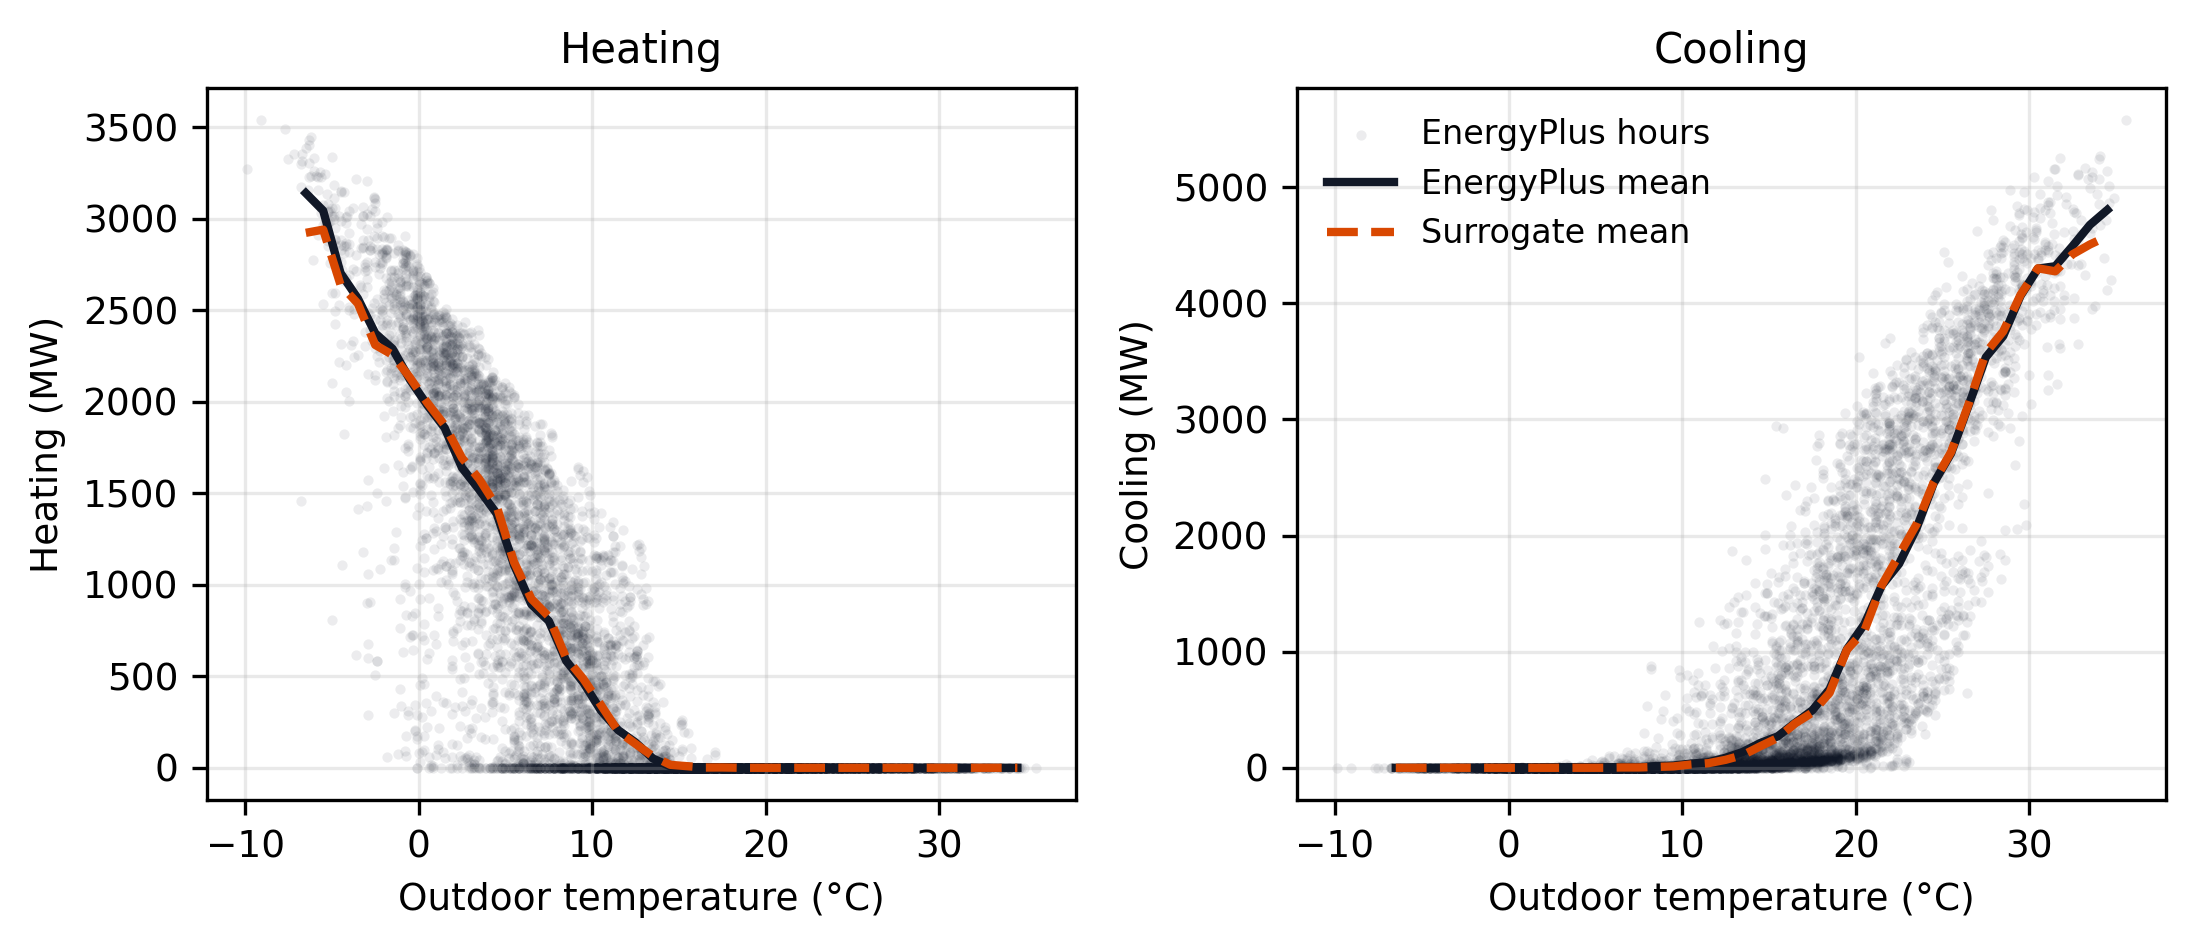
\includegraphics[width=0.92\textwidth]{fig_03_temperature_response.png}
\caption{Floor-area-weighted Vienna heating and cooling demand as a function
of outdoor temperature. Points show hourly EnergyPlus values. Lines show
EnergyPlus and surrogate means in 1-K temperature bins with at least eight
observations.}
\label{fig:temperature}
\end{figure*}

EnergyPlus produces \SI{0.43}{\giga\watt\hour} of heating from June through
August, compared with \SI{1.84}{\giga\watt\hour} from the surrogate. This
residual is small relative to the approximately \SI{5.3}{\tera\watt\hour}
annual EnergyPlus space-heating series, but it indicates that the on/off
transition is not reproduced perfectly.

\subsection{Computational Performance}

The complete EnergyPlus demand path takes \SI{67.1}{\second}, including
\SI{27.5}{\second} for input preparation, \SI{24.8}{\second} for the simulation
engine, and \SI{14.8}{\second} for SQL extraction
(Table~\ref{tab:runtime}). Surrogate inference for both targets takes
\SI{1.73}{\second}, corresponding to a speedup of 38.8. Engine wall-clock time
alone is 14.3 times the inference time. The one-time fit of both surrogate
models requires \SI{18.5}{\second}.

\begin{table}[t]
\centering
\caption{Runtime for eight cohorts and 8760 hours.}
\label{tab:runtime}
\small
\begin{tabular}{lrrrr}
\toprule
Path & Prep. & Engine & SQL & Total \\
 & [s] & [s] & [s] & [s] \\
\midrule
EnergyPlus & 27.5 & 24.8 & 14.8 & 67.1 \\
Surrogate inference & -- & -- & -- & 1.73 \\
\bottomrule
\end{tabular}
\end{table}

The inference comparison assumes that the hourly input table is available;
loading and preparing a new weather table are not included. For repeated
evaluations, 50 city years would require approximately \SI{3355}{\second} on
the EnergyPlus path and \SI{87}{\second} for surrogate inference, a difference
of about \SI{55}{\minute}.

\section{Discussion}

The results show that a compact statistical model can retain most of the
hourly variation generated by the EnergyPlus cohort simulations. Annual
energy and temporal correlation are reproduced more accurately than the
maximum load. This distinction matters for energy-system applications. The
surrogate is suitable for producing hourly demand shapes that are subsequently
normalized to an independently specified annual energy balance. It should not
be used without qualification when the EnergyPlus maximum itself is treated as
a design load.

The city-level results describe all floor area in the Citiwatts inventory, but
they do not resolve every building in Vienna. Buildings within a given sector
and construction period share one equivalent archetype and one operating
profile. Aggregation therefore retains major differences in envelope quality
while suppressing variations in geometry, occupancy, refurbishment state, and
control behaviour within each cohort. The non-residential archetypes carry
additional uncertainty because Vienna-specific geometry and window data were
not available at the same level as for Austrian residential apartment
buildings.

The validation is deliberately separated in time: complete calendar weeks are
excluded from each fit. It is nevertheless limited to one weather year and to
the same eight cohorts used during training. The reported accuracy therefore
supports interpolation across unseen periods of 2023, but not transfer to a
different climate, an extreme year outside the training range, or an unseen
building type. The remaining underestimation of peak loads is consistent with
this limitation.

Finally, the surrogate reproduces reference heating and cooling demand only.
It does not contain setpoint changes, preheating, load curtailment, rebound, or
indoor-temperature state transitions. These processes require a separate
stateful response model before building flexibility can be represented in an
optimization problem.

\section{Conclusions}

An EnergyPlus-to-surrogate workflow was developed for hourly useful heating
and cooling demand of the Vienna building stock. Eight archetypes represent
the complete Citiwatts floor area across two sectors and four construction
periods. Their EnergyPlus outputs form a 70,080-row annual data set. Separate
histogram gradient-boosting hurdle models reproduce held-out cohort-hour
demand with $R^2$ values of 0.959 for heating and 0.975 for cooling.

After aggregation to the Vienna stock, annual errors remain below 2\%, while
peak loads are underestimated by 7--10\%. Surrogate inference is approximately
39 times faster than the complete EnergyPlus demand path. The resulting model
provides a computationally efficient source of EnergyPlus-consistent demand
profiles for subsequent energy-system analyses, provided that annual energy
anchors and peak-load limitations remain explicit.

\balance
\begin{thebibliography}{12}

\bibitem{crawley2001}
D.B. Crawley, L.K. Lawrie, F.C. Winkelmann, W.F. Buhl, Y.J. Huang,
C.O. Pedersen, R.K. Strand, R.J. Liesen, D.E. Fisher, M.J. Witte, and
J. Glazer, ``EnergyPlus: creating a new-generation building energy simulation
program,'' \emph{Energy and Buildings}, vol. 33, pp. 319--331, 2001.

\bibitem{doe2026}
U.S. Department of Energy, \emph{EnergyPlus Version 26.1.0 Documentation},
2026.

\bibitem{westermann2019}
P. Westermann and R. Evins, ``Surrogate modelling for sustainable building
design---A review,'' \emph{Renewable and Sustainable Energy Reviews},
vol. 110, pp. 440--450, 2019.

\bibitem{amasyali2018}
K. Amasyali and N.M. El-Gohary, ``A review of data-driven building energy
consumption prediction studies,'' \emph{Renewable and Sustainable Energy
Reviews}, vol. 81, pp. 1192--1205, 2018.

\bibitem{citiwatts2026}
Citiwatts, ``Urban energy and building-stock indicators for Vienna,'' 2026.
[Online]. Available: \url{https://citiwatts.eu/}

\bibitem{loga2016}
T. Loga, B. Stein, and N. Diefenbach, ``TABULA building typologies in 20
European countries---Making energy-related features of residential building
stocks comparable,'' \emph{Energy and Buildings}, vol. 132, pp. 4--12, 2016.

\bibitem{aea2012}
Austrian Energy Agency, \emph{TABULA National Scientific Report Austria},
2012. [Online]. Available:
\url{https://episcope.eu/fileadmin/tabula/public/docs/scientific/AT_TABULA_ScientificReport_AEA.pdf}

\bibitem{zippenfenig2023}
P. Zippenfenig, ``Open-Meteo.com Weather API,'' Zenodo, 2023. [Online].
Available: \url{https://open-meteo.com/}

\bibitem{climateonebuilding}
Climate.OneBuilding, ``AUT Vienna Innere Stadt weather files.'' [Online].
Available: \url{https://climate.onebuilding.org/}

\bibitem{friedman2001}
J.H. Friedman, ``Greedy function approximation: a gradient boosting machine,''
\emph{The Annals of Statistics}, vol. 29, pp. 1189--1232, 2001.

\bibitem{pedregosa2011}
F. Pedregosa et al., ``Scikit-learn: Machine learning in Python,''
\emph{Journal of Machine Learning Research}, vol. 12, pp. 2825--2830, 2011.

\bibitem{ke2017}
G. Ke, Q. Meng, T. Finley, T. Wang, W. Chen, W. Ma, Q. Ye, and T.-Y. Liu,
``LightGBM: A highly efficient gradient boosting decision tree,'' in
\emph{Advances in Neural Information Processing Systems 30}, 2017.

\end{thebibliography}

\end{document}
